\documentclass[a4paper,english, 10pt, twoside]{article}
\usepackage[utf8]{inputenc}
\usepackage[T1]{fontenc}
\usepackage[english]{babel}
\usepackage{epsfig}
\usepackage{graphicx}
\usepackage{amsfonts, amssymb, amsmath}
\usepackage{listings}
\usepackage{float}
\usepackage[top=2cm, bottom=2cm, left=2cm, right=2cm]{geometry}

%opening
\title{Project 2, FYS4150}
\author{Fredrik E Pettersen\\ fredriep@student.matnat.uio.no}


\begin{document}

\maketitle

\begin{abstract}

\end{abstract}

\section*{About the problem}
In this project we will study two electrons trapped in a three dimensional harmonic oscillator well, with and without the repulsive
Coloumb force interaction. We will model the problem with the Schrödinger equation assuming spherical symmetry, and hopefully we
will end up reproducing the results from the article...
To solve the problems we need to rewrite the Schrödinger equation to a form which is more managable. Starting off with the 
assumption of spherical symmetry we can simplify
\begin{align*}
\frac{-\hbar^2}{2m}\nabla^2\Psi +V\Psi &= i\hbar\frac{\partial}{\partial t}\Psi\\
\frac{-\hbar^2}{2m}\left(\frac{1}{r^2}\frac{d}{dr}r^2\frac{d}{dr}-\frac{l(l+1)}{r^2}\right)R(r) &+V(r)R(r) = ER(r)
\end{align*}
In our case $V(r)$ is the harmonic oscillator potential $\frac{1}{2}kr^2$ with $k = m\omega^2$ and E is the
energy of the harmonic oscillator in three dimensions. The oscillator frequency is $\omega$ and
the energies are
$$
E_{n,l} = \left(2n+l+\frac{3}{2}\right)
$$
with $n = 0,1,2...$ and $l = 0,1,2,...$ and $r\in[0,\infty)$\\
The quantum number l is the orbital momentum of the electron. Proceding now, we substitute $R(r) = \frac{u(r)}{r}$, and look at
the case of $l=0$.
\begin{align*}
r\frac{-\hbar^2}{2m}\left(\frac{1}{r^2}\frac{d}{dr}r^2\frac{d}{dr}\right)\frac{u(r)}{r} +V(r)u(r) = Eu(r)\\
\frac{-\hbar^2}{2m}\left(\frac{1}{r}\frac{d}{dr}\frac{r^2}{r^2}\left[\frac{du(r)}{dr}r - u(r)\right]\right) +V(r)u(r) = Eu(r)\\
\frac{-\hbar^2}{2m}\left[\frac{d^2u(r)}{dr^2} + \frac{du(r)}{dr} - \frac{du(r)}{dr} \right] +V(r)u(r) = Eu(r)\\
\end{align*}
We now set $\rho = \frac{r}{\alpha}$ and insert for the potential $V(\rho) = \frac{1}{2}k\alpha^2\rho^2$.
\begin{align*}
\frac{-\hbar^2}{2m\alpha^2}\frac{d^2u(\rho)}{d\rho^2} +V(\rho)u(\rho) = Eu(\rho)\\
\frac{-\hbar^2}{2m\alpha^2}\frac{d^2u(\rho)}{d\rho^2} +\frac{1}{2}k\alpha^2\rho^2u(\rho) = Eu(\rho)\\
-\frac{d^2u(\rho)}{d\rho^2} + \frac{k\alpha^4m}{\hbar^2}\rho^2 = \frac{2m\alpha^2}{\hbar^2}Eu(\rho)
\end{align*}
Defining $\alpha^4 = \frac{\hbar^2}{km}$ and $\lambda = \frac{2m\alpha^2}{\hbar^2}E$ leaves us with
$$
-\frac{d^2}{d\rho^2}u(\rho) + \rho^2u(\rho) = \lambda u(\rho)
$$
Which has the eigenvalues $\lambda_0 = 3$, $\lambda_1 = 7$, $\lambda_2 = 11$ and higher for $l=0$. Using the standard approximation
for the second derivative
$$
u''(\rho) \simeq \frac{u(\rho -h) -2u(\rho) + u(\rho+h)}{h^2} = \frac{u_{i+1} - 2u_i + u_{i-1}}{h^2}
$$
where $h = \frac{\rho_{max} - \rho_0}{n+1}$ and $u_i$ denotes the i'th element in u which is $u(\rho +i*h)$, we discretize the 
problem. As an additional approximation we need to limit $\rho_{max}$. The physical limits of this 
system are $\rho_{max} \to \infty$ and $u(0) = u(\infty) = 0$, but obviously we cannot simulate forever. Our best hope is to set
some limit to $\rho_{max}$ and hope that $u(\rho_{max}) \simeq 0$ within some reasonable limit (say $u(\rho_{max}) = 10^{-10}$ or 
less). This discretization gives us the following form of the Schrödinger equation
$$
\frac{2u_i -u_{i-1} - u_{i+1}}{h^2} + \rho_i^2u_i = \lambda u_i
$$
which we can set up as a matrix problem just like in project 1. Resulting in:
\begin{align*}
&A \vec{x} = \lambda \vec{x} \\
A =   &\left( \begin{array}{ccccccc} \frac{2}{h^2}+V_1 & -\frac{1}{h^2} & 0   & 0    & \dots  &0     & 0 \\
                                -\frac{1}{h^2} & \frac{2}{h^2}+V_2 & -\frac{1}{h^2} & 0    & \dots  &0     &0 \\
                                0   & -\frac{1}{h^2} & \frac{2}{h^2}+V_3 & -\frac{1}{h^2}  &0       &\dots & 0\\
                                \dots  & \dots & \dots & \dots  &\dots      &\dots & \dots\\
                                0   & \dots & \dots & \dots  &\dots       &\frac{2}{h^2}+V_{n_{\mathrm{step}}-2} & -\frac{1}{h^2}\\
                                0   & \dots & \dots & \dots  &\dots       &-\frac{1}{h^2} & \frac{2}{h^2}+V_{n_{\mathrm{step}}-1}
             \end{array} \right)  
\end{align*}
Notice the indeces ranging from 1 to $n_{step}-1$. The funtion values at the indeces $n_{step}=0$ and $n_{step}=n$ are the 
 boundary conditions which are left out of the calculations. $\vec{x}$ is an eigenvector of A (denoting an eigenfunction).\\
 
When we later add the Coloumb interaction between the two electrons we will be left with a very similar expression. Starting off 
with the radial Schrödinger equation we add another electron like so:
\begin{align*}
 \frac{-\hbar^2}{2m}\frac{d^2}{dr^2}u(r) + \frac{1}{2}kr^2u(r) = E^{(1)}u(r)\\
 \left(-\frac{\hbar^2}{2m}\frac{d^2}{dr_1^2} -\frac{\hbar^2}{2m}\frac{d^2}{dr_2^2}+ \frac{1}{2}kr_1^2 + \frac{1}{2}kr_2^2\right)
 u(r_1,r_2) = E^{(2)}u(r_1,r_2)\\
\end{align*}
This equation is without the Coloumb repulsion, and contains the two-particle wavefunction $u(r_1,r_2)$ and two particle energy
$E^{(2)}$. Introducing a relative coordinate $\mathbf{r} = r_2 - r_1$ beeing the relative distance between the electrons, and a 
center of mass coordinate $R = \frac{r_1 + r_2}{2}$ the equation reads
\begin{align*}
\left( -\frac{\hbar^2}{m} \frac{d^2}{dr^2} -\frac{\hbar^2}{4m} \frac{d^2}{R^2}+ \frac{1}{4}kr^2 + kR_2^2\right)
u(r,R) = E^{(2)}u(r,R)
\end{align*}
and we separate this by assuming that $u(r,R) = \psi(r)\phi(R)$ which makes the total energy $E^{(2)} = E_r + E_R$.
We now add the Coloumb interaction between the two electrons by adding the term 
$$
V(r_1,r_2) = \frac{\beta e^2}{\left|\mathbf{r_2}-\mathbf{r_1}\right|} = \frac{\beta e^2}{r}
$$
to the potential. Doing this makes our equation
$$
\left( \frac{-\hbar^2}{m}\frac{d^2}{dr^2} + \frac{1}{4}kr^2\ + \frac{\beta e^2}{r}\right)\psi(r) = E_r\psi(r)
$$
Which is very similar to the equation without Coloumb interaction. If we again introduce $\rho = \frac{r}{\alpha}$ and normalize 
we get
\begin{align*}
 -\frac{d^2}{d\rho^2}\psi(\rho) +\frac{mk}{4\hbar^2}\alpha^4\rho^2\psi(\rho) + \frac{m\alpha\beta e^2}{\rho\hbar^2}\psi(\rho) 
 = \frac{m\alpha^2}{\hbar^2} E_{\rho}\psi(\rho)\\
 -\frac{d^2}{d\rho^2}\psi(\rho) +\omega_r^2\rho^2\psi(\rho) + \frac{1}{\rho}\psi(\rho)  = \lambda\psi(\rho)\\
\end{align*}
where we have defined $\alpha = \frac{\hbar^2}{m\beta e^2}$, $\lambda = \frac{m\alpha^2}{\hbar^2}E_{\rho}$ and 
$\omega_r^2 = \frac{mk\alpha^4}{4\hbar^2}$. We also ommit the center of mass energy.
Notice that with a smart structure in the program to solve this, we only need to add 
the new potential in order to solve the new problem. 

\section*{The algorithm}
Unlike project 1 this is an eigenvalue problem, meaning that we need
to use a different algorithm to solve it. Because it is a very intuitive algorithm we will solve the problem by Jacobi's rotation
method. The mentality of this method is to perform successive similarity transformations of the matrix where we try to zero out a 
nondiagonal element in each transformation. The way we zero out an element is, as the name suggests, by multiplying our matrix with
a rotation matrix and its inverse (which is also its transpose), rotating our matrix an angle $\theta$ each time like this.
\begin{align*}
A\vec{x} &= \lambda\vec{x}\\
R^T_1AR_1\vec{x} &= R^T_1\lambda\vec{x}R_1 = \lambda R^T_1\vec{x}R_1 = \lambda \vec{x'}\\
R^T_2R^T_1AR_1R_2\vec{x} &= \lambda\vec{x''}\\
...\\
R^T_nR^T_{n-1}\cdots R^T_1AR_1\cdots R_n\vec{x} &= \lambda\vec{x'^n}\\
\end{align*}
\begin{align*}
R = \left(\begin{array}{cccccccc}
           1 & 0 & \dots & 0 & \dots & 0 & 0 & 0\\
	   0 & 1 & 0 & \dots & 0 & \dots & 0 & 0\\
	   \dots & 0 & \dots & \dots &0 & \dots & \dots & 0\\
	   0 & \dots & \dots & cos(\theta) & 0 & \dots  & 0 & sin(\theta)\\
	   0 & 0 & \dots & 0 & 1 & 0 & \dots & 0 \\
	   \dots & 0 & \dots & \dots & 0 & \dots & 0 & 0\\
	   0 & 0 & \dots  & 0  & 0 & \dots & 1 & 0\\
	   0 & \dots & 0 & -sin(\theta) & 0 & \dots & 0 & cos(\theta)
          \end{array}\right)
\end{align*}
Now this will converge to a diagonal matrix, but in order to finish we will be happy when all nondiagonal elements are less than 
some $\epsilon$.\\


When doing the multiplication of the matrices in the Jacobi rotation we make a new matrix $B = R^TAR$. This matrix has the elemets 
\begin{align*}
 b_{ii} &= a_{ii},\; i\neq k,\, i\neq l\\
 b_{ik} &= a_{ik}cos(\theta) - a_{il}sin(\theta), \: i\neq k,\, i\neq l\\
 b_{il} &= a_{il}cos(\theta + a_{ik}sin(\theta),\: i\neq k,\, i\neq l\\
 b_{kk} &= a_{kk}cos^2(\theta) - 2a_{kl}cos(\theta)sin(\theta) + a_{ll}sin^2(\theta)\\
 b_{ll} &= a_{ll}cos^2(\theta) + 2a_{kl}cos(\theta)sin(\theta) + a_{kk}sin^2(\theta)\\
 b_{kl} &= (a_{kk} - a_{ll})cos(\theta)sin(\theta) + a_{kl}(cos^2(\theta) - sin^2(\theta))\\
\end{align*}
Where $a_{lk}=a_{kl}$ is the larges nondiagonal element of A.
What we wish to do is simply setting the elements $b_{kl} = a_{kl}$ and $b_{lk} = a_{lk}$ to zero and change the diagonal while 
the rest of the elements are unchanged. The price we pay for doing is to also change $b_{ik}$ and $b_{il}$. We can minimize the 
damage done to these elements by choosing the smallest possible angle, making $cos(\theta) \simeq 1$ and $sin(\theta) \simeq 0$. 
Now, the way we calculate our $sin(\theta)$ and $cos(\theta)$ is through
$$
\tau = cot(2\theta) = \frac{a_{ll}-a{kk}}{2a{kl}}, \; tan(\theta) = -\tau \pm \sqrt{1+\tau^2}
$$
As we all know, $tan(\theta) = \frac{sin(\theta)}{cos(\theta)}$. So if $tan(\theta)$ is as small as possible, $sin(\theta)$ must 
be as small as possible. Now, we can safely assume that $\left|\tau\right|>1$ because the diagonal elements of A are all larger 
than the nondiagonal elements, and we are seeking to diagonalize A. Thus $\left|\tau\right|$ will steadily become larger during 
the calculations. Looking at the expression $tan(\theta) = -\tau\pm \sqrt{1+\tau^2}$ we see that:
\begin{align*}
\lim_{\left|\tau\right|\to\infty} -\tau\pm \sqrt{1+\tau^2} = 1\\
\left|tan(\theta)\right| = 1 \implies \left|\theta\right|\leq \frac{\pi}{4}
\end{align*}
Now, the part which does the actual rotations in my code is the function ``rotate'', based heavily on the same function in the 
lecture notes. This function looks a bit cryptic at first glance, so I'll go through it step by step here.
\lstinputlisting{algo.txt}
As we will se in the section about results, Jacobis algorithm requires $\propto n^2$ rotations of the matrix A to give sufficently 
accurate results. This does not sound to bad in the begining, but looking at the algorithm, each rotation is something like 
$18n + 30$ FLOPS including square roots, pluss 3 if tests which are slow. And in addition to this we need to find the largest 
element in A after each rotation which is another $\frac{n^2}{2}$ FLOPS and if-tests. So in total we end up with $n^4$ FLOPS, tests 
and square roots to get a usable result. This is not exactly good. A better way to get the results we want is to use is to directly 
calculate the eigenvalues directly from our tridiagonal matrix by Francis' algorithm. In the recourse file on the webpage of the 
course we find this algorithm implemented, and thus we only need to modify it to use armadillo objects.

\section*{Analytic solution}
The problem with confining two interacing electrons in a harmonic oscillator well has an analytic solution described in M.Taut's 
article plblished in November 1993. Mr Taut starts off by doing more or less the same assumptions and rewrites as we have done in 
the introduction, but with a lot more reasoning. He is left with the same equation for the Coloub interacting case, only differing 
by a factor of $\frac{1}{2}$. Meaning that our results are the double of Tauts results. \\
\section*{Results}
Having run the Jacobi-rotation algorithm for increasing values of n and $\rho_{max}$ in the intervals $n \in [50,100,150,...,700]$
and $\rho_{max}\in [4,5,...15]$ it seems that the optimal combination of $\rho_{max}$ and n in order to get the three lowest 
eigenvalues with 4 leading digits is $n=650,\rho_{max} = 5$. In order to get the lowest eigenvalue with 4 leading digits we only
need $n = 200, \rho_{max} = 4$. All of the simulations have been run with $\epsilon = 10^{-6}$.
To make alle the nondiagonal matrix elements numerically zero (that is smaller than $10^{-16}$) it seems like we need to run 
something like $2.05\cdot n^2$ rotations. As a comparison I have extracted the number of rotations as a function of n for the seemingly most 
accurate value of $\rho_{max}$ to be approximately $1.565\cdot n^2$.
\begin{center}
\begin{figure}[H]
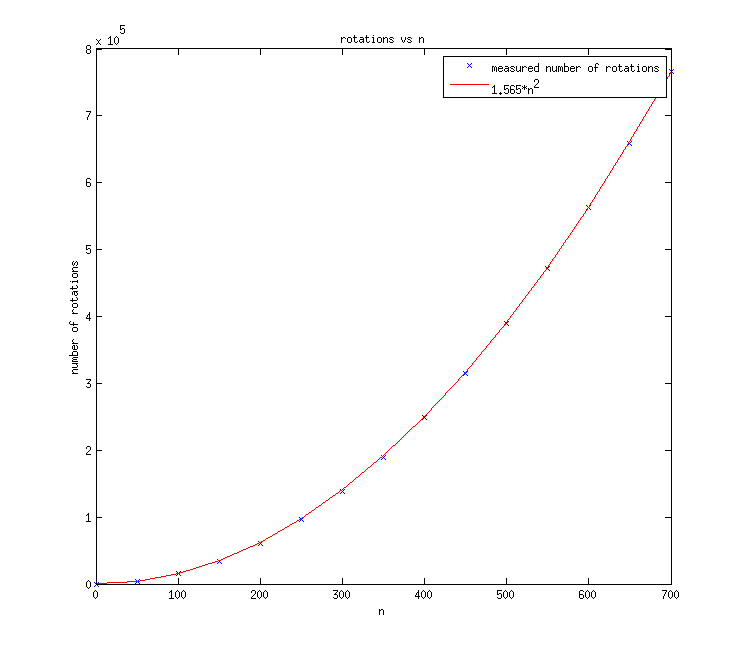
\includegraphics[scale = 0.6]{nsquared1.png}
\caption{Number of rotations by Jacobis method as function on N. $\rho_{max}=5$ and $\epsilon = 10^{-6}$ used.}
\end{figure}
\end{center}

\begin{center}
\begin{figure}[H]
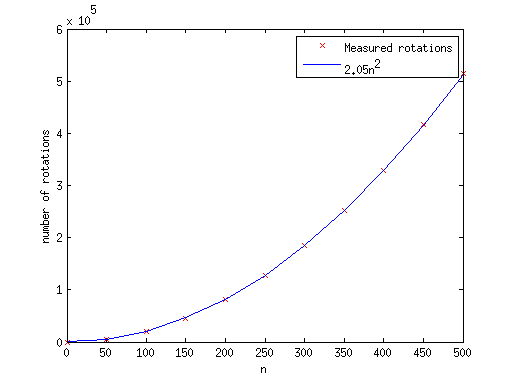
\includegraphics[scale = 0.7]{num_zero.png}
\caption{Number of rotations by Jacobis method as function on N. $\rho_{max}=5$ and $\epsilon = 10^{-16}$ used.}
\end{figure}
\end{center}

As a sidestep I'd like to compare the efficiency of Jacobis algorithm and Fancis' algorithm. When I ran my script for the Jacobi 
algoritgm I saved information about the time it took to run each program. I will use the mean of these values, and when comparing 
with Francis' algorithm.
\begin{table}[H]
\begin{center}
\begin{tabular}{|c|c|c|}
\hline N & Jacobi time & Francis time\\
\hline 50 & 50 & 10\\
\hline 100 & 730 & 40\\
\hline 150 & 3 400 & 110\\
\hline 200 & 11 000 & 260\\
\hline 300 & 58 000 & 900\\
\hline 400 & 190 000 & 2 000\\
\hline 500 & 425 000 & 4 000\\
\hline 600 & 910 000 & 6 800\\
\hline 700 & 1 830 000 & 11 000\\
\hline
\end{tabular}
\caption{Approximate mean CPU time in milliseconds for Jacobi and Francis algorithms.}
\end{center}
\end{table}

And now we come to the real reason we have done all of this. Using Francis' algorithm (which gives the same results as my 
implementation of Jacobis algorithm only faster) I have calculated the eigenvectors of the three lowest energy states. The 
eigenvectors correspond to the eigenfunctions of the system, and these are plotted below. Of course, varying the oscillator frequency
$\omega_r$ has an impact on where we can cut off our calculations (or where we can set infinity to be). To get a fairly good 
result I have done the simulations with $N = 700$, remember we only got 4 leading digits on all three eigenvalues with $N > 650$ 
for Jacobis method, and increased $\rho_{max}$ until another increase in $\rho_{max}$ gives the same 3 or more decimals in the 
eigenvalues. Remember that a small value of $\omega_r$ indicates a weak oscillator which in turn lets the electrons go further away 
from the origin. 

\begin{center}
\begin{figure}[H]
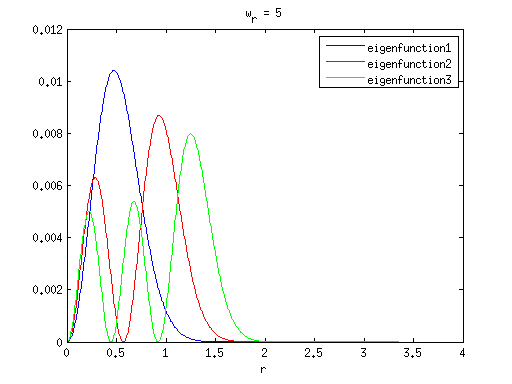
\includegraphics[scale = 0.7]{plot_c_n700_rhomax4_omega_5.png}
\caption{Eigenfunctions plotted vs $\rho$. $N = 700$}
\end{figure}
\end{center}

\begin{center}
\begin{figure}[H]
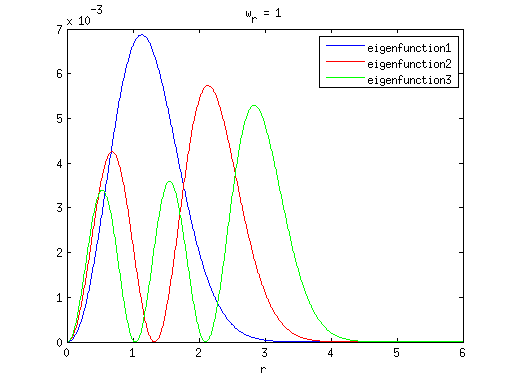
\includegraphics[scale = 0.7]{plot_c_n700_rhomax6_omega_1.png}
\caption{Eigenfunctions plotted vs $\rho$. $N = 700$}
\end{figure}
\end{center}

\begin{center}
\begin{figure}[H]
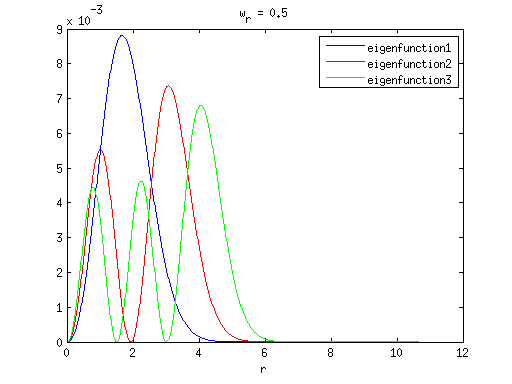
\includegraphics[scale = 0.7]{plot_c_n700_rhomax11_omega_05.png}
\caption{Eigenfunctions plotted vs $\rho$. $N = 700$}
\end{figure}
\end{center}

\begin{center}
\begin{figure}[H]
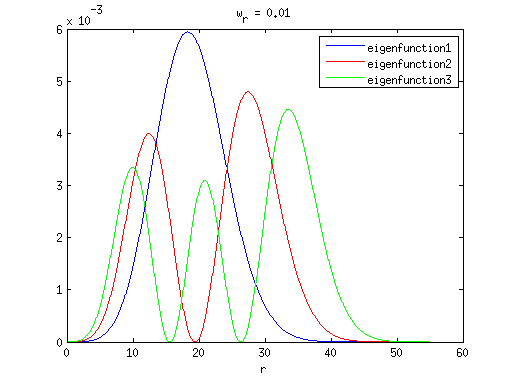
\includegraphics[scale = 0.7]{plot_c_n700_rhoma551_omega_001.png}
\caption{Eigenfunctions plotted vs $\rho$. $N = 700$}
\end{figure}
\end{center}
I must say that the eigenfunctions look almost suspiciously alike...
What we can say with certainty is that the stronger (larger) the oscillator frecuency, the closer to the origin we find the two 
electrons. However, the second and third energystate seems to have a larger probability further away from the origin than close 
to it.
\section*{Stability and precision}
I have not been able to get hold of more the eigenvalues with more than 5 digits for some reason, but still I would like to say 
something about the importance of the $\epsilon$ parameter. First of all, the correct way to run Jacobis algorithm is to run until 
$$
\left(2\cdot\Sigma_{j>i}A_{i,j}^2\right)^{1/2} <\epsilon
$$
and specify some $\epsilon$. This means that all the nondiagonal matrix elements are numerically zero, or zero for all practical 
purposes. However, doing this sum of squares and sqare root operations becomes very time consuming. In fact I ran my program which 
implemented this simultaniously as another student who only checked if the largest nondiagonal element in A was smaller than 
$\epsilon$. We sent the same parameters in and got the same results (within the precision we could get out), but my program ran 
for almost 10 minutes longer. Thus I have left the sum of sqares out of my program.\\
Beeing curious about the importance of $\epsilon$ I ran some tests for $\epsilon = [10,1,0.1,...10^{-11}]$ with the results 
listed in figure. As we can see (and again, I only have acces to 5 leading digits) even with $\epsilon=0.1$ we get decent 
precision. Figure lists the relative error compared with the CPU-time used to do the computations. What I'd like to point out is 
that the relative error seems to decrease rapidly in the beginning and then flat out. So in case the error should continue to decrease 
at the pace it does in the beginning, an $\epsilon$ of $10^{-6}$ will make the error of order $\epsilon_r < 10^{-8}$. If the error 
does in fact reach some limit, wich it seems to do, the gain on decreasing $\epsilon$ further than $10^{-6}$ is so small compared 
to the increase in CPU-time spent that it is simply not worth it.\\
\begin{center}
\begin{figure}[H]
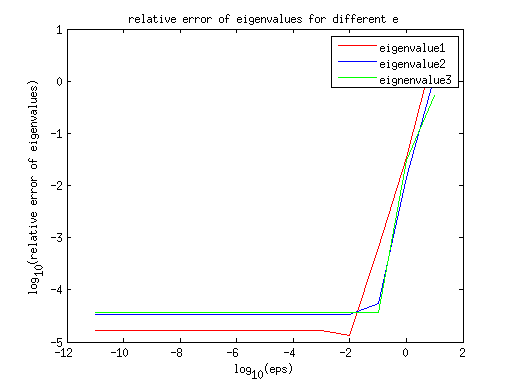
\includegraphics[scale = 0.7]{relative_error.png}
\caption{The relative error of eigenvalues for different $\epsilon$. }
\end{figure}
\end{center}
\begin{center}
\begin{figure}[H]
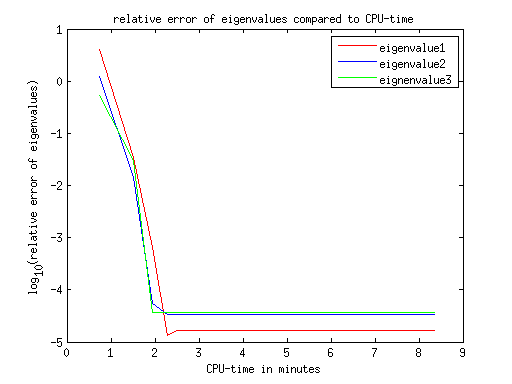
\includegraphics[scale = 0.5]{num_zero_time.png}
\caption{The relative error of eigenvalues compared to the CPU-time used to produce them. }
\end{figure}
\end{center}

\section*{Source code}
I have created the programs listed in the appendix in order to do the required simulations. The functions ``rotate'' and ``tqli'' 
are based heavily on exisiting code from the textbook and the file lib.cpp on the course homepage. Theese are, however, modified 
to use armadillo objects such as mat and vec. Unlike the C++ convention I have gathered all of my functions in the header file 
jacobi.h. I do this because I think it makes the overall program more readable.
To get hold of the eigenvectors corresponding to the lowest energy states we need to sort the columns in the matrix ``z'' returned 
from the function ``tqli''. This is done by first sorting the vector containing the eigenvalues, and keeping the indeces of the 
eigenvalues while sorting them. These indeces correspond to the indeces of the columns in z which are the eigenvectors. 

I have also made a simple script to check which combinations of n and $\rho_{max}$ produce the best results. I would like to 
mention that my executable file is named ``goggen''.
%\lstinputlisting{proj2script.m}
%\lstinputlisting{jacobi.cpp}
%\lstinputlisting{jacobi.h}
\section*{Final comments}
If there is one thing I have learned from this project it is that Jacobis algorithm, while simple and fairly easy to program, is 
a stupidly slow algorithm. It is especially stupid to apply to any tridiagonal problem because we can rather use Francis method to 
acquire the eigenvalues and eigenvectors.\\

\end{document}
